\documentclass[11pt]{article}
\usepackage[a4paper, margin=1.54cm]{geometry}
\usepackage[utf8]{inputenc}
\usepackage{babel}
\usepackage[spanish]{layout}
\usepackage[article]{ragged2e}
\usepackage{textcomp}
\usepackage{amsmath}
\usepackage{amssymb}
\usepackage{amsfonts}
\usepackage{proof}
\usepackage{enumerate}
\usepackage{graphicx}
\usepackage{multirow}
\usepackage{caption}
\usepackage{subcaption}
\usepackage{blkarray, bigstrut}
\def\Big#1{\makebox(0,0){\huge#1}}

\setlength{\parindent}{0pt}

\title{
    Trabajo Práctico Machine Learning \\
    \large Introducción a la Inteligencia Artificial}
\author{Mellino, Natalia \and Farizano, Juan Ignacio}

\date{}

\begin{document}
\maketitle

\noindent\rule{\textwidth}{1pt}

\section*{Introducción al dataset}

Trabajaremos sobre el conjunto de datos \emph{yeast} donde entrenaremos
a nuestros modelos para que clasifiquen distintos tipos de levadura. \\

Este dataset consta de 9 atributos, el primero es simplemente un nombre de
secuencia y por lo tanto se ignora ya que no tiene relevancia.
Los restantes atributos son: MCG, GVH, ALM, MIT, ERL, POX, VAC, y NUC. \\

Cada instancia será clasificada en alguna de las siguientes 10 clases, donde 
originalmente en los datos dados se distribuyen de la siguiente manera: 

\begin{table}[h!]
  \begin{center}
    \begin{tabular}{|c|c|}
      \hline
      Clase     & Cantidad     \\ \hline
      CYT       & 463          \\ \hline
      NUC       & 429          \\ \hline
      MIT       & 244          \\ \hline
      ME3       & 163          \\ \hline
      ME2       & 51           \\ \hline
      ME1       & 44           \\ \hline
      EXC       & 37           \\ \hline
      VAC       & 30           \\ \hline
      POX       & 20           \\ \hline
      ERL       & 5            \\ \hline
    \end{tabular}
  \end{center}
\end{table}

Cargamos estos datos en R para poder trabajar con ellos y borramos la primer
columna ya que es del atributo no relevante.
\begin{verbatim}
  yeast <- read.table("yeast.data", header = FALSE, col.names = c("sname", "mcg", "gvh",
     "alm", "mit", "erl", "pox", "vac", "nuc", "type"))
  yeast <- yeast[, -1]
\end{verbatim}

\section*{Entrenamiento del modelo}

Al entrenar el modelo, utilizamos el método de \emph{k-fold cross validation},
donde elegimos un $k$ igual a 5 para obtener nuestros conjuntos de entrenamiento
y testeo. \\

\begin{verbatim}
indexData <- createFolds(t(yeast[, "type"]), k = 5)
kElegido <- 3
yeastTest <- yeast[indexData[[kElegido]], ]
yeastTrain <- yeast[setdiff(seq(1:dim(yeast)[1]), indexData[[kElegido]]), ]
\end{verbatim}

\subsection*{Utilizando Ganancia de Información}

Una vez obtenidos estos conjuntos, procedemos a crear nuestros árboles de 
decisión utilizando la librería \emph{rpart} y su función homónima. \\

En primera instancia, como criterio elegido para dividir los nodos utilizamos el 
método de Ganancia de Información.

\begin{verbatim}
fitGain <- rpart(type~., data = yeastTrain, parms = list(split = 'information'))
fancyRpartPlot(fitGain, caption = NULL)
\end{verbatim}

Obtenemos el siguiente árbol:

\begin{figure}[h!]
  \begin{center}
    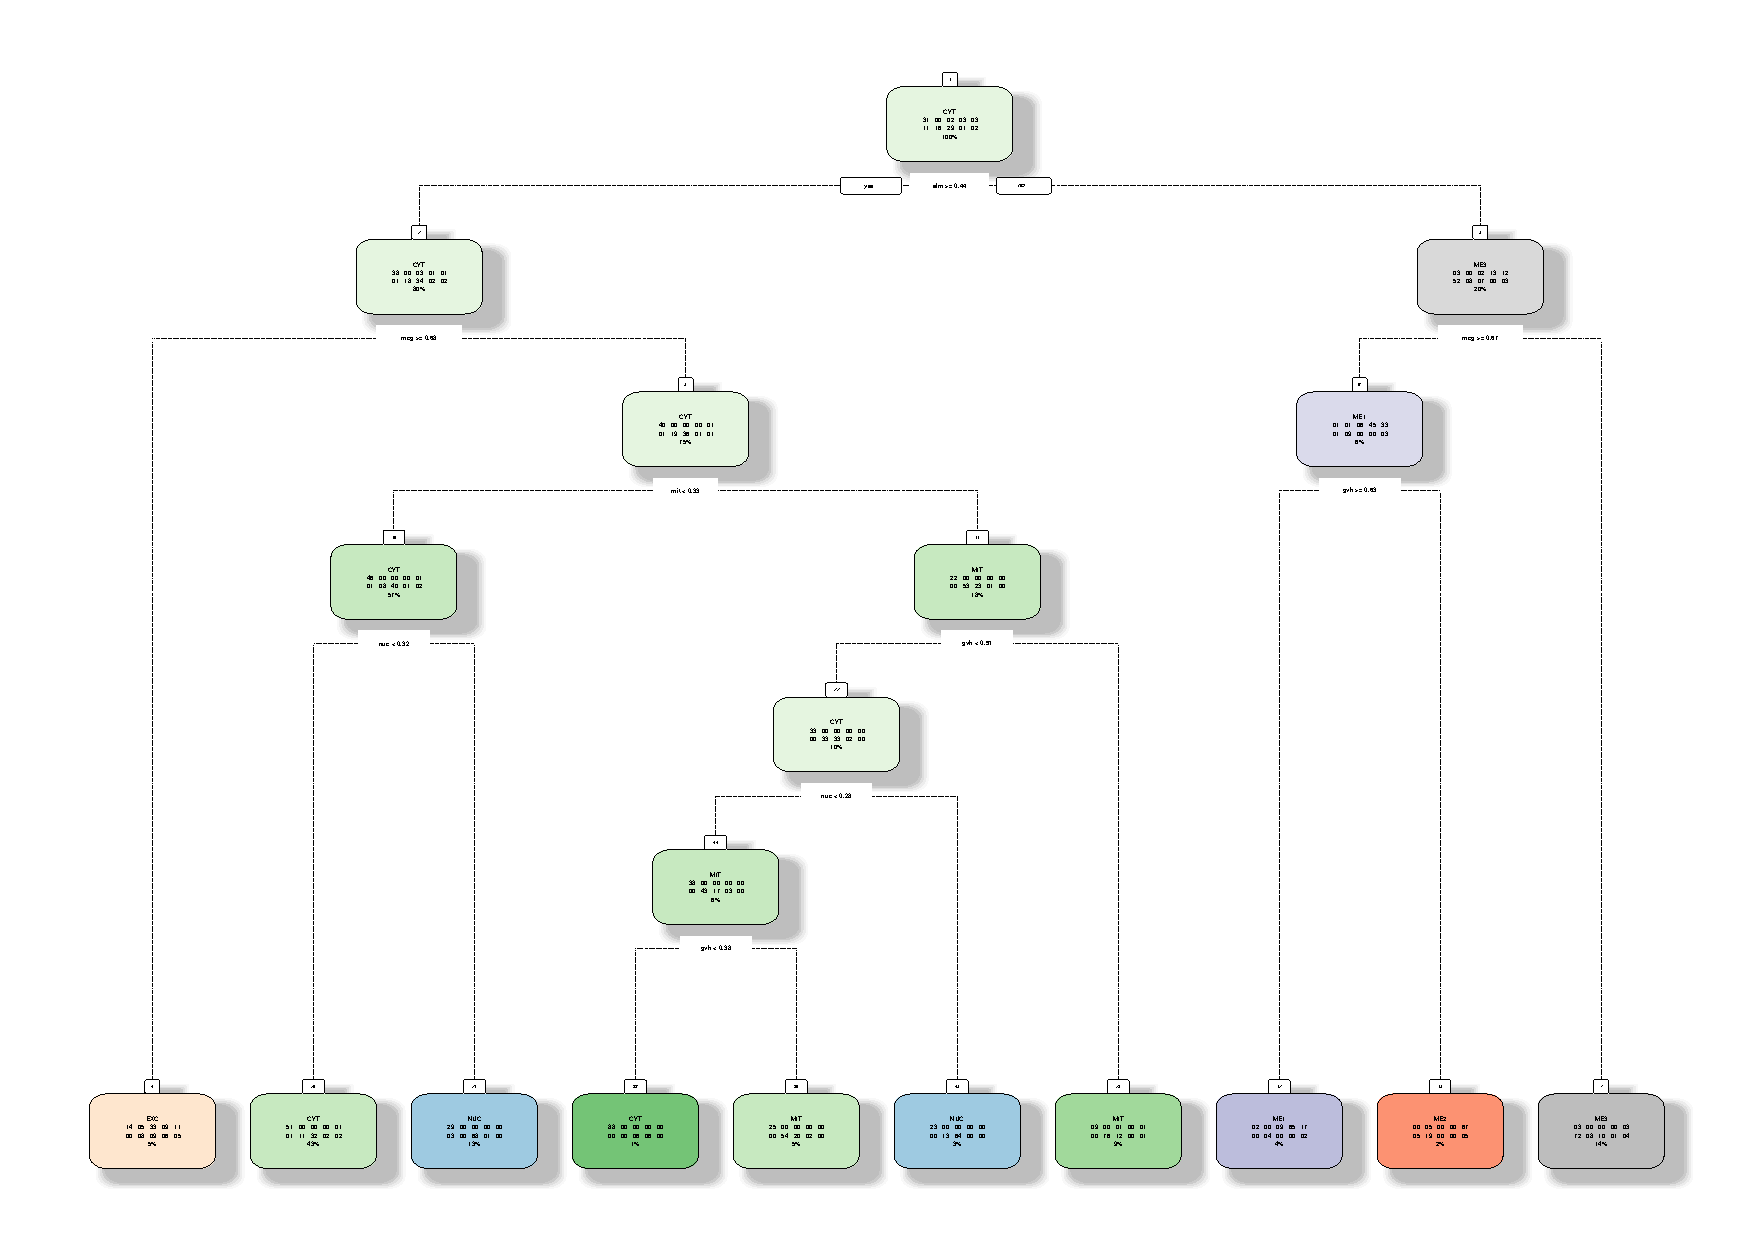
\includegraphics[width=1\linewidth]{treeGain.pdf}
  \end{center}
\end{figure}

Una vez obtenido el árbol, lo ponemos a prueba con nuestro conjunto de testeo.

\begin{verbatim}
predictYeastGain <- predict(fitGain, yeastTest[,-9], type = 'class')
\end{verbatim}

A partir de estos resultados, podemos armar la siguiente matriz de confusión:
\begin{verbatim}
  matrixGain <- table(predictYeastGain, yeastTest[,9])
\end{verbatim}

\begin{equation*}
  \begin{blockarray}{ccccccccccc}
     & \text{CYT} &  \text{ERL} & \text{EXC} & \text{ME1} & \text{ME2} & \text{ME3} & \text{MIT} & \text{NUC} & \text{POX} & \text{VAC} \\
    \begin{block}{c(cccccccccc)} 
      \text{CYT} & 70 & 0 & 2 & 0 & 0 &  1 & 13 & 42 &  3 & 2 \\
      \text{ERL} &  0 & 0 & 0 & 0 & 0 &  0 &  0 &  0 &  0 & 0 \\
      \text{EXC} &  4 & 1 & 4 & 2 & 3 &  0 &  3 &  2 &  1 & 3 \\
      \text{ME1} &  0 & 0 & 1 & 6 & 0 &  0 &  0 &  0 &  0 & 0 \\
      \text{ME2} &  0 & 0 & 0 & 0 & 6 &  0 &  1 &  1 &  0 & 0 \\
      \text{ME3} &  3 & 0 & 0 & 0 & 1 & 29 &  5 &  4 &  0 & 1 \\
      \text{MIT} &  8 & 0 & 0 & 0 & 0 &  0 & 24 &  3 &  0 & 0 \\
      \text{NUC} &  8 & 0 & 0 & 0 & 0 &  2 &  3 & 34 &  0 & 0 \\
      \text{POX} &  0 & 0 & 0 & 0 & 0 &  0 &  0 &  0 &  0 & 0 \\
      \text{VAC} &  0 & 0 & 0 & 0 & 0 &  0 &  0 &  0 &  0 & 0 \\
    \end{block}
  \end{blockarray}
\end{equation*}

\subsubsection*{Métricas}

Utilizando el siguiente código en R calculamos los valores correspondientes a 
Accuracy, Precision y Recall. Para Precision y Recall calculamos los promedios utilizando
el valor asociado a cada clase, reemplazando los NaN por 0.

\begin{verbatim}
  # Accuracy 
  acuraccyGain <- sum(diag(matrixGain)) / sum(matrixGain)

  # Precision
  precisionGain <- diag(matrixGain) / rowSums(matrixGain)
  precisionGain[is.nan(precisionGain)] <- 0 # Reemplazamos los NaN por 0 para el promedio
  
  # Recall
  recallGain <- diag(matrixGain) / colSums(matrixGain)
  recallGain[is.nan(recallGain)] <- 0

  # Juntamos las métricas en una sola tabla
  measuresGain <- rbind(acuraccyGain, mean(precisionGain), mean(recallGain))
  rownames(measuresGain) <- c("acuraccy", "precision", "recall")
\end{verbatim}

Los resultados obtenidos son los siguientes:

\begin{table}[h!]
  \begin{center}
    \begin{tabular}{|c|c|}
      \hline
      Métrica     & Valor     \\ \hline
      Accuracy    & 0.584     \\ \hline
      Precision   & 0.439     \\ \hline
      Recall      & 0.446     \\ \hline
    \end{tabular}
  \end{center}
\end{table}

Podemos observar más en detalle los valores obtenidos para Precision y Recall en cada clase:

\begin{table}[h!]
  \begin{center}
    \begin{tabular}{|c|c|c|c|c|c|c|c|c|c|c|}
      \hline
      Métrica/Clase  & CYT    & ERL & EXC   & ME1    & ME2  & ME3   & MIT   & NUC   & POX & VAC \\ \hline
      Precision      & 0.526  & 0   & 0.173 & 0.857  & 0.75 & 0.674 & 0.685 & 0.723 &  0  & 0   \\ \hline
      Recall         & 0.752  & 0   & 0.571 & 0.750  & 0.60 & 0.906 & 0.489 & 0.395 &  0  & 0   \\ \hline
    \end{tabular}
  \end{center}
\end{table}

\subsection*{Utilizando el método de Gini}

Para el método de Gini el análisis se realiza de la misma forma que en la sección anterior.

\begin{verbatim}
fitGini <- rpart(type~., data = yeastTrain, parms = list(split = 'gini'))
fancyRpartPlot(fitGini, caption = NULL)
\end{verbatim}

\begin{figure}[h!]
  \begin{center}
    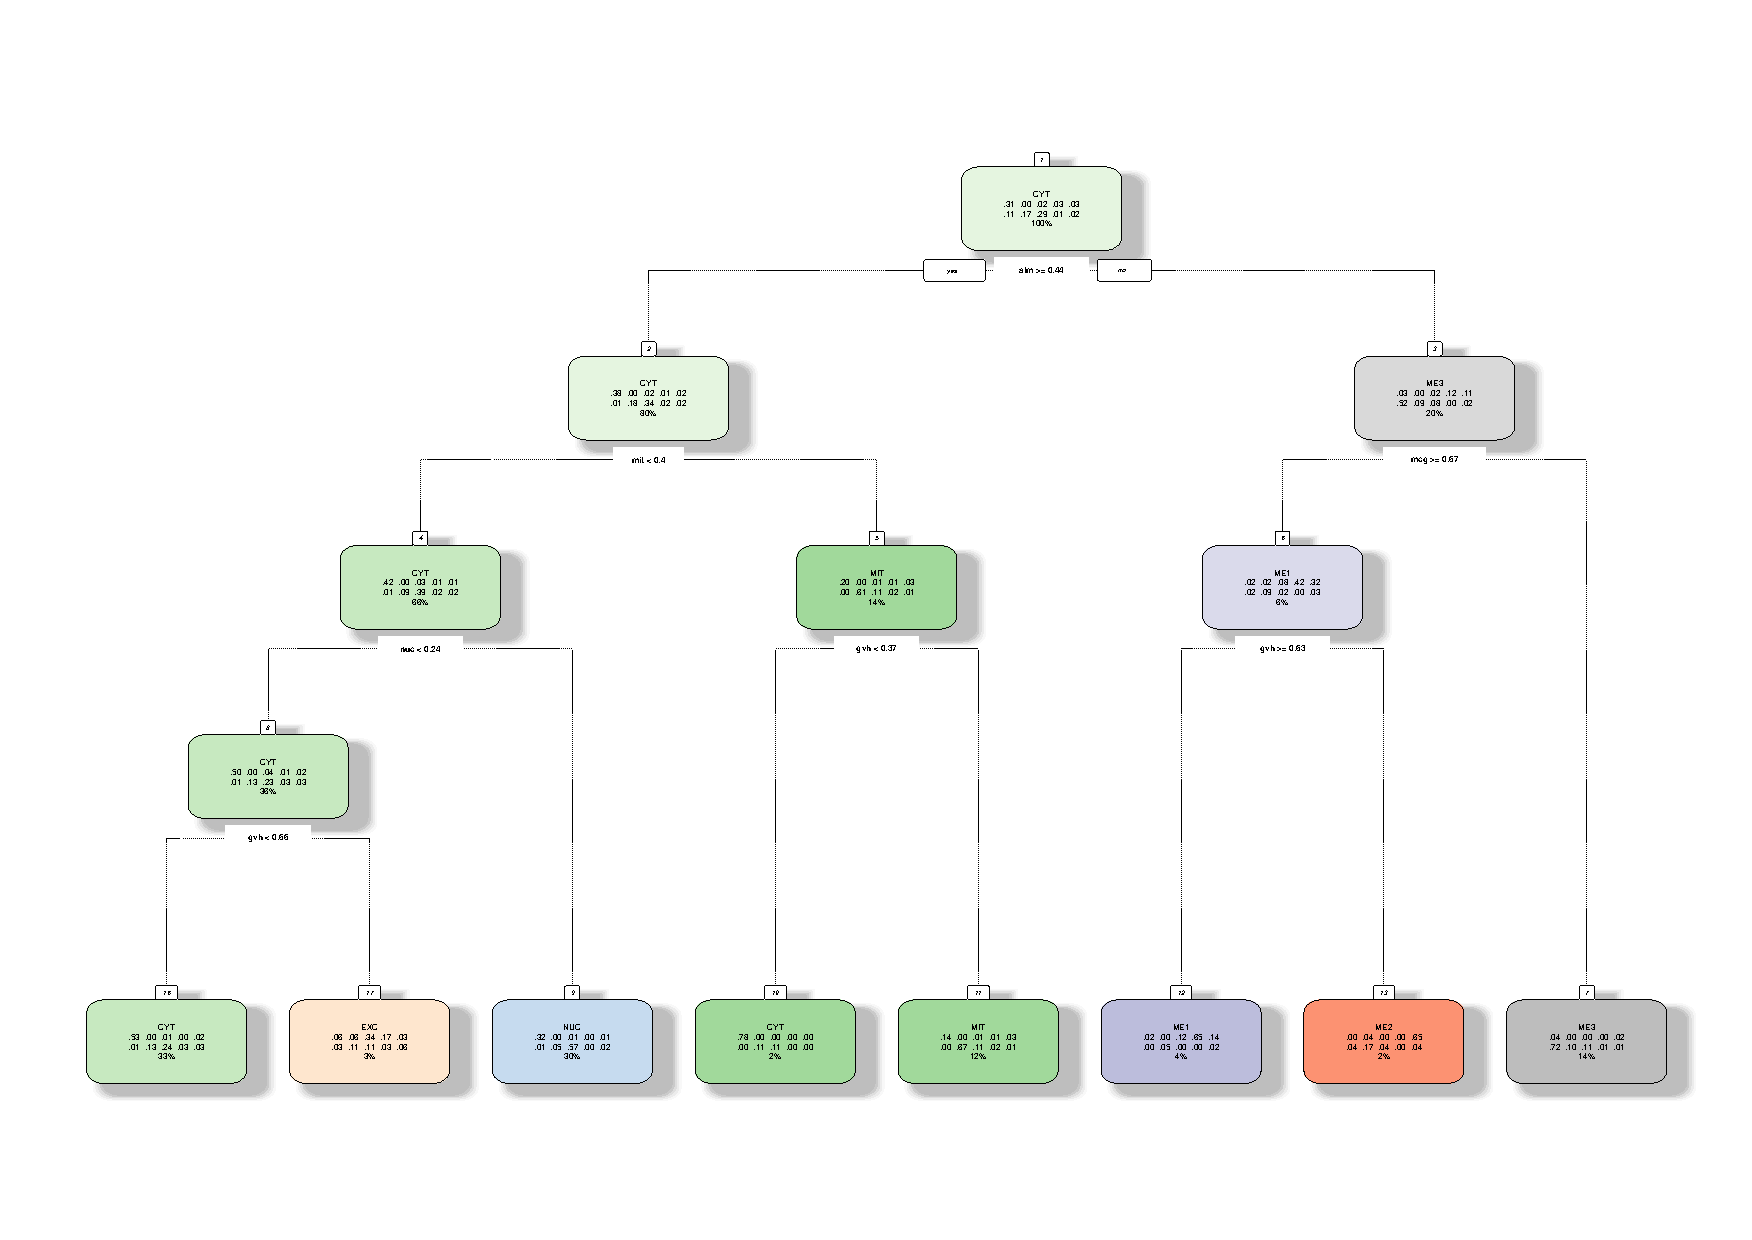
\includegraphics[width=1\linewidth]{treeGini.pdf}
  \end{center}
\end{figure}

\begin{verbatim}
predictYeastGini <- predict(fitGini, yeastTest[,-9], type = 'class')
matrixGini <- table(predictYeastGini, yeastTest[,9])  
\end{verbatim}

\begin{equation*}
  \begin{blockarray}{ccccccccccc}
     & \text{CYT} &  \text{ERL} & \text{EXC} & \text{ME1} & \text{ME2} & \text{ME3} & \text{MIT} & \text{NUC} & \text{POX} & \text{VAC} \\
    \begin{block}{c(cccccccccc)} 
      \text{CYT} & 58 & 1 & 4 & 0 & 1 &  1  & 18  & 32 & 3 & 4 \\
      \text{ERL} &  0 & 0 & 0 & 0 & 0 &  0  &  0  &  0 & 0 & 0 \\
      \text{EXC} &  2 & 0 & 2 & 2 & 0 &  0  &  0  &  0 & 0 & 1 \\
      \text{ME1} &  0 & 0 & 1 & 6 & 0 &  0  &  0  &  0 & 0 & 0 \\
      \text{ME2} &  0 & 0 & 0 & 0 & 6 &  0  &  1  &  1 & 0 & 0 \\
      \text{ME3} &  3 & 0 & 0 & 0 & 1 & 29  &  5  &  4 & 0 & 1 \\
      \text{MIT} &  6 & 0 & 0 & 0 & 2 &  0  & 24  &  2 & 1 & 0 \\
      \text{NUC} & 24 & 0 & 0 & 0 & 0 &  2  &  1  & 47 & 0 & 0 \\
      \text{POX} &  0 & 0 & 0 & 0 & 0 &  0  &  0  &  0 & 0 & 0 \\
      \text{VAC} &  0 & 0 & 0 & 0 & 0 &  0  &  0  &  0 & 0 & 0 \\
    \end{block}
  \end{blockarray}
\end{equation*}

\begin{verbatim}
  # Accuracy 
  acuraccyGini <- sum(diag(matrixGini)) / sum(matrixGini)

  # Precision
  precisionGini <- diag(matrixGini) / rowSums(matrixGini)
  precisionGini[is.nan(precisionGini)] <- 0 # Reemplazamos los NaN por 0 para el promedio
  
  # Recall
  recallGini <- diag(matrixGini) / colSums(matrixGini)
  recallGini[is.nan(recallGini)] <- 0

  # Juntamos las métricas en una sola tabla
  measuresGini <- rbind(acuraccyGini, mean(precisionGini), mean(recallGini))
  rownames(measuresGini) <- c("acuraccy", "precision", "recall")
\end{verbatim}

\begin{table}[h!]
  \begin{center}
    \begin{tabular}{|c|c|}
      \hline
      Métrica     & Valor     \\ \hline
      Accuracy    & 0.581     \\ \hline
      Precision   & 0.436     \\ \hline
      Recall      & 0.420     \\ \hline
    \end{tabular}
  \end{center}
\end{table}

Podemos observar más en detalle los valores obtenidos para Precision y Recall en cada clase:

\begin{table}[h!]
  \begin{center}
    \begin{tabular}{|c|c|c|c|c|c|c|c|c|c|c|}
      \hline
      Métrica/Clase & CYT    & ERL & EXC   & ME1  & ME2   & ME3   & MIT   & NUC   & POX & VAC \\ \hline
      Precision     & 0.475  & 0   & 0.285 & 0.857 & 0.75 & 0.674 & 0.685 & 0.635 & 0   &  0  \\ \hline
      Recall        & 0.623  & 0   & 0.285 & 0.750 & 0.60 & 0.906 & 0.489 & 0.546 & 0   &  0  \\ \hline
    \end{tabular}
  \end{center}
\end{table}

\section*{Conclusiones}

\begin{itemize}
  \item Los datos no estaban bien distribuidos, para algunas clases había muy
  pocas instancias, lo cual contribuyó a que el modelo no pueda inferir sobre las mismas.
  \item Las métricas obtenidas al testear los árboles obtenidos con ambos criterios son muy pobres,
  esto nos da indicios de que no pueden ser utilizados para clasificar correctamente 
  de forma confiable, lo que nos lleva a pensar que los árboles de decisión no son
  un modelo apropiado para este dataset.
  \item Se intentó realizar la poda de los árboles, pero los resultados de acuerdo
  a las métricas vistas anteriormente eran inferiores por lo que nos quedamos
  con los árboles originales sin realizarse poda.
  \item La diferencia entre las métricas de los testeos de los árboles obtenidos
  por ganancia de información y por impureza de Gini se encuentran dentro
  del margen de error, por lo que un método no resulta realmente superior sobre el otro,
  es indistinto cual se elija.
  \item En los resultados obtenidos tanto con ganancía de información como con impureza de Gini, podemos
  ver que las clases ME1, ME2 y ME3 presentan mayor Precision y Recall por sobre las demás, incluso
  por sobre las clases CYT y NUC que son las que más instancias tenían. Por lo que
  podemos pensar que son las clases más diferenciables de las demás según los atributos.
  \item Para las clases ERL, POX, y VAC las métricas no son concluyentes debido a la poca cantidad
  de ejemplares que presenta el dataset, por lo que nuestro modelo no puede clasificar en estas clases.
  \item Al ser un dominio muy específico sobre el cual no tenemos conocimientos y además
  al tener información compleja, no podemos analizar en detalles los resultados.
\end{itemize}

\end{document}